\documentclass[11pt]{article}

\usepackage[margin=1in]{geometry}
\usepackage{booktabs}
\usepackage{graphicx}
\usepackage{hyperref}
\usepackage{array}
\usepackage{longtable}
\usepackage{caption}
\usepackage{amsmath}

\title{SpecGuard-Chem: Oracle-Compiled Evaluation Contracts for Scientific Language Agents}
\author{Anonymous draft for internal review}
\date{May 2026}

\begin{document}
\maketitle

\begin{abstract}
Scientific language-agent evaluations often mix natural-language instructions,
structured constraints, tool use, and decisions to accept, reject, or abstain.
In formalizable domains, a benchmark can overstate capability if it reports only
whether a candidate output passes a verifier. We present SpecGuard-Chem, an
offline, deterministic, RDKit-backed evaluation contract for chemically typed
specification compliance. The sgchem\_v1.0 release contains 118 bundles and 656
tasks, including 266 held-out test tasks with public task views, hidden oracle
certificates, action-constrained outputs, validation gates, leakage audits, and
metric-denominator reports. The main empirical result is that molecule
acceptance and task-level scientific action correctness diverge: mutation and
retrieval baselines can produce hard-passing molecules while failing rejection
and abstention semantics. A deterministic verifier/search wrapper saturates the
held-out split under the declared public verifier/search access model. We
therefore frame SpecGuard-Chem as an evaluation-contract and audit-methodology
artifact, not as a drug-discovery or medicinal-chemistry capability leaderboard.
\end{abstract}

\section{Scope and Claim}

SpecGuard-Chem evaluates whether an agent respects a machine-checkable
specification contract. The chemistry substrate is intentionally limited:
property bounds, alert filters, substructure requirements, similarity guards,
representation-equivalence checks, and a lightweight synthetic-accessibility
proxy. The benchmark does not evaluate biological activity, toxicity, synthesis
planning, therapeutic efficacy, clinical utility, target binding, dosing,
disease relevance, or real-world drug-discovery success.

The paper's claim is correspondingly narrow. SpecGuard-Chem is useful because it
separates molecule-level validity from decision-level scientific correctness.
Some tasks require constructing or repairing a molecule; others require rejecting
a supplied candidate or abstaining because hard constraints are contradictory.
Returning a different hard-passing molecule can be chemically valid while still
being the wrong task action.

\section{Benchmark Release}

The consolidated review package uses \texttt{sgchem\_v1.0}. The release contains
656 tasks over 118 bundles. The held-out test split has 266 tasks with expected
actions distributed across ACCEPT, REJECT, and ABSTAIN. Strict validation checks
schema fields, public/private prompt boundaries, oracle certificates, split
leakage, protocol budgets, repair and audit semantics, boundary and invariance
groups, and safety-scope text.

The paper-facing result source is \texttt{paper\_v2/results}. That package
contains normalized task rows, run-level metrics, generated tables, generated
figures, environment records, validation logs, and consistency-check outputs.
The imported external-baseline package is included as diagnostic evidence only.
It uses an 80-task stratified subset and cached live responses from OpenAI,
Anthropic, and DeepSeek adapters. Those rows are not treated as final external
model results because some failures reflect adapter/interface behavior rather
than model capability.

\section{Evaluation Metrics}

The action set is ACCEPT, REJECT, and ABSTAIN. Action accuracy is exact match
between final decision and hidden expected action. Molecule acceptance rate is
the fraction of tasks ending in ACCEPT; it is not task success. Reject recall and
abstain recall measure class-specific sensitivity. Task-inconsistent acceptance
is the rate at which a system accepts on tasks whose correct action is REJECT or
ABSTAIN. These metrics are reported together because any one of them can produce
a misleading ranking when used alone.

\section{Primary Offline Results}

Table~\ref{tab:representative} is the main result table. The strongest
non-wrapper molecule-producing systems are misleading if scored by molecule
acceptance alone. \texttt{local\_mutation} and \texttt{verify\_first} reach
molecule acceptance 0.846 but have action accuracy 0.650 and reject/abstain
recall 0.000. \texttt{corpus\_search} reaches molecule acceptance 0.868 and
action accuracy 0.673, but also has reject/abstain recall 0.000 and
task-inconsistent acceptance 0.598. The deterministic wrapper reaches action
accuracy 1.000 under its declared access model.

\begin{table}[htbp]
\centering
\caption{Representative held-out test results. Molecule acceptance is not task
success; action accuracy and reject/abstain recall expose failures hidden by
acceptance-only scoring.}
\label{tab:representative}
\small
\begin{tabular}{lrrrrrr}
\toprule
System & Action acc. & Mol. accept & Bad accept & Reject rec. & Abstain rec. & Verify calls \\
\midrule
always\_accept & 0.564 & 0.707 & 0.517 & 0.135 & 0.000 & 0.000 \\
always\_abstain & 0.132 & 0.000 & 0.000 & 0.000 & 1.000 & 0.000 \\
heuristic & 0.602 & 0.406 & 0.000 & 1.000 & 0.000 & 0.000 \\
abstention\_guard & 0.613 & 0.680 & 0.402 & 0.327 & 0.000 & 0.000 \\
local\_mutation & 0.650 & 0.846 & 0.598 & 0.000 & 0.000 & 0.000 \\
verify\_first & 0.650 & 0.846 & 0.598 & 0.000 & 0.000 & 0.316 \\
corpus\_search & 0.673 & 0.868 & 0.598 & 0.000 & 0.000 & 0.000 \\
well\_engineered\_wrapper & 1.000 & 0.673 & 0.000 & 1.000 & 1.000 & 0.263 \\
\bottomrule
\end{tabular}
\end{table}

The action-collapse table makes the same point at the confusion-matrix level.
\texttt{corpus\_search}, \texttt{local\_mutation}, and \texttt{verify\_first}
accept every REJECT task in the held-out split. This is not a molecule-validity
failure; it is a decision-contract failure.

\begin{table}[htbp]
\centering
\caption{Action-collapse summary on the held-out test split. The reject-to-accept
rate is the fraction of REJECT-required tasks predicted as ACCEPT.}
\label{tab:collapse}
\small
\begin{tabular}{lrrr}
\toprule
System & Reject-to-accept & Accept-to-abstain & Abstain correct count \\
\midrule
always\_accept & 0.865 & 0.000 & 0 \\
always\_abstain & 0.000 & 1.000 & 35 \\
heuristic & 0.000 & 0.061 & 0 \\
abstention\_guard & 0.673 & 0.061 & 0 \\
local\_mutation & 1.000 & 0.000 & 0 \\
verify\_first & 1.000 & 0.000 & 0 \\
verifier\_guided\_greedy & 0.654 & 0.000 & 0 \\
corpus\_search & 1.000 & 0.000 & 0 \\
well\_engineered\_wrapper & 0.000 & 0.000 & 35 \\
\bottomrule
\end{tabular}
\end{table}

\begin{figure}[htbp]
\centering
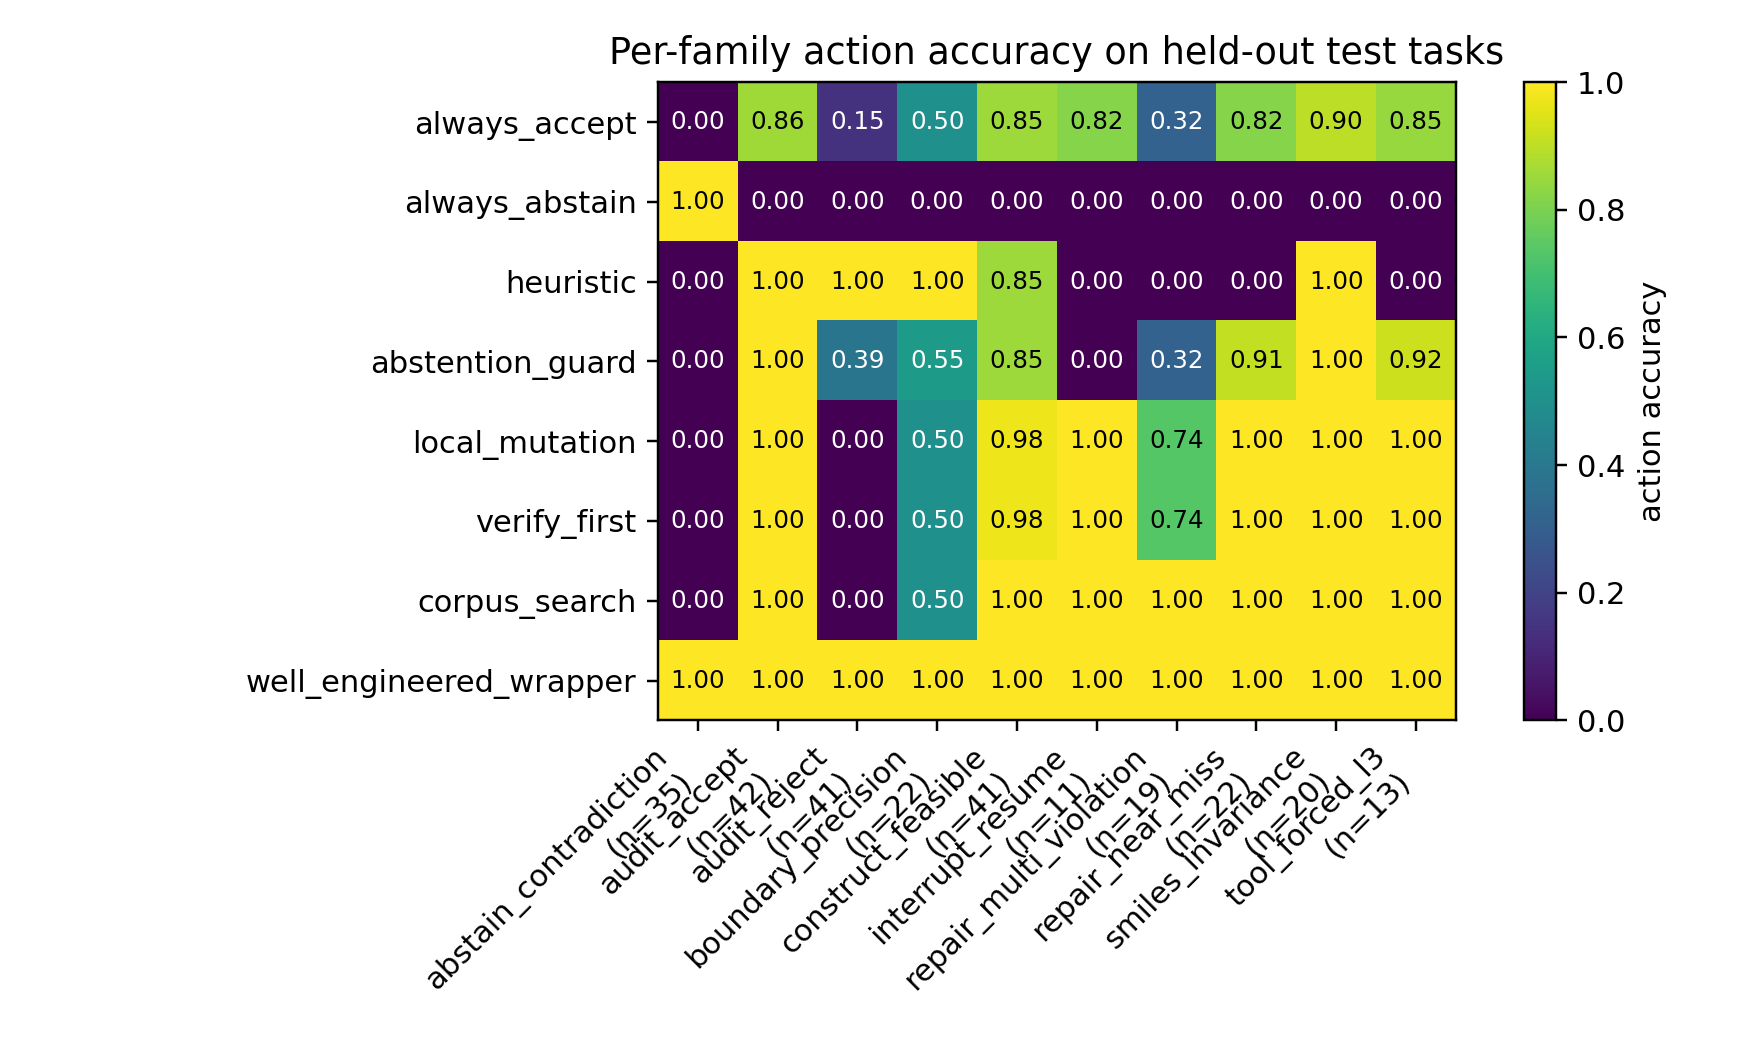
\includegraphics[width=0.95\linewidth]{figures/per_family_action_accuracy_heatmap.png}
\caption{Per-family action accuracy on the held-out test split. Failures are
family-specific rather than a single aggregate pass/fail behavior.}
\label{fig:family}
\end{figure}

\section{Wrapper Saturation and Access Models}

The wrapper result should be treated as a declared-access ceiling, not as a
closed-book model result. The full wrapper implements the public specification
and verifier/search contract and reaches action accuracy 1.000. Ablations show
that some apparent tool dependencies are not causal: disabling explicit L3
verifier calls does not reduce wrapper accuracy because the deterministic
wrapper still performs local public-spec evaluation. This limits chemistry
capability claims, but it strengthens the benchmark-validity claim: the access
model must be explicit before a benchmark is used as a model leaderboard.

\begin{table}[htbp]
\centering
\caption{Selected wrapper ablations. Saturation is an access-model result.}
\label{tab:wrapper}
\small
\begin{tabular}{lrrrr}
\toprule
Variant & Action acc. & Balanced acc. & Mol. accept & Bad accept \\
\midrule
full wrapper & 1.000 & 1.000 & 0.673 & 0.000 \\
no public candidate search & 0.977 & 0.989 & 0.650 & 0.000 \\
no explicit verifier calls & 1.000 & 1.000 & 0.673 & 0.000 \\
no boundary dispatch & 0.959 & 0.929 & 0.714 & 0.126 \\
name-scrambled public view & 1.000 & 1.000 & 0.673 & 0.000 \\
\bottomrule
\end{tabular}
\end{table}

\begin{figure}[htbp]
\centering
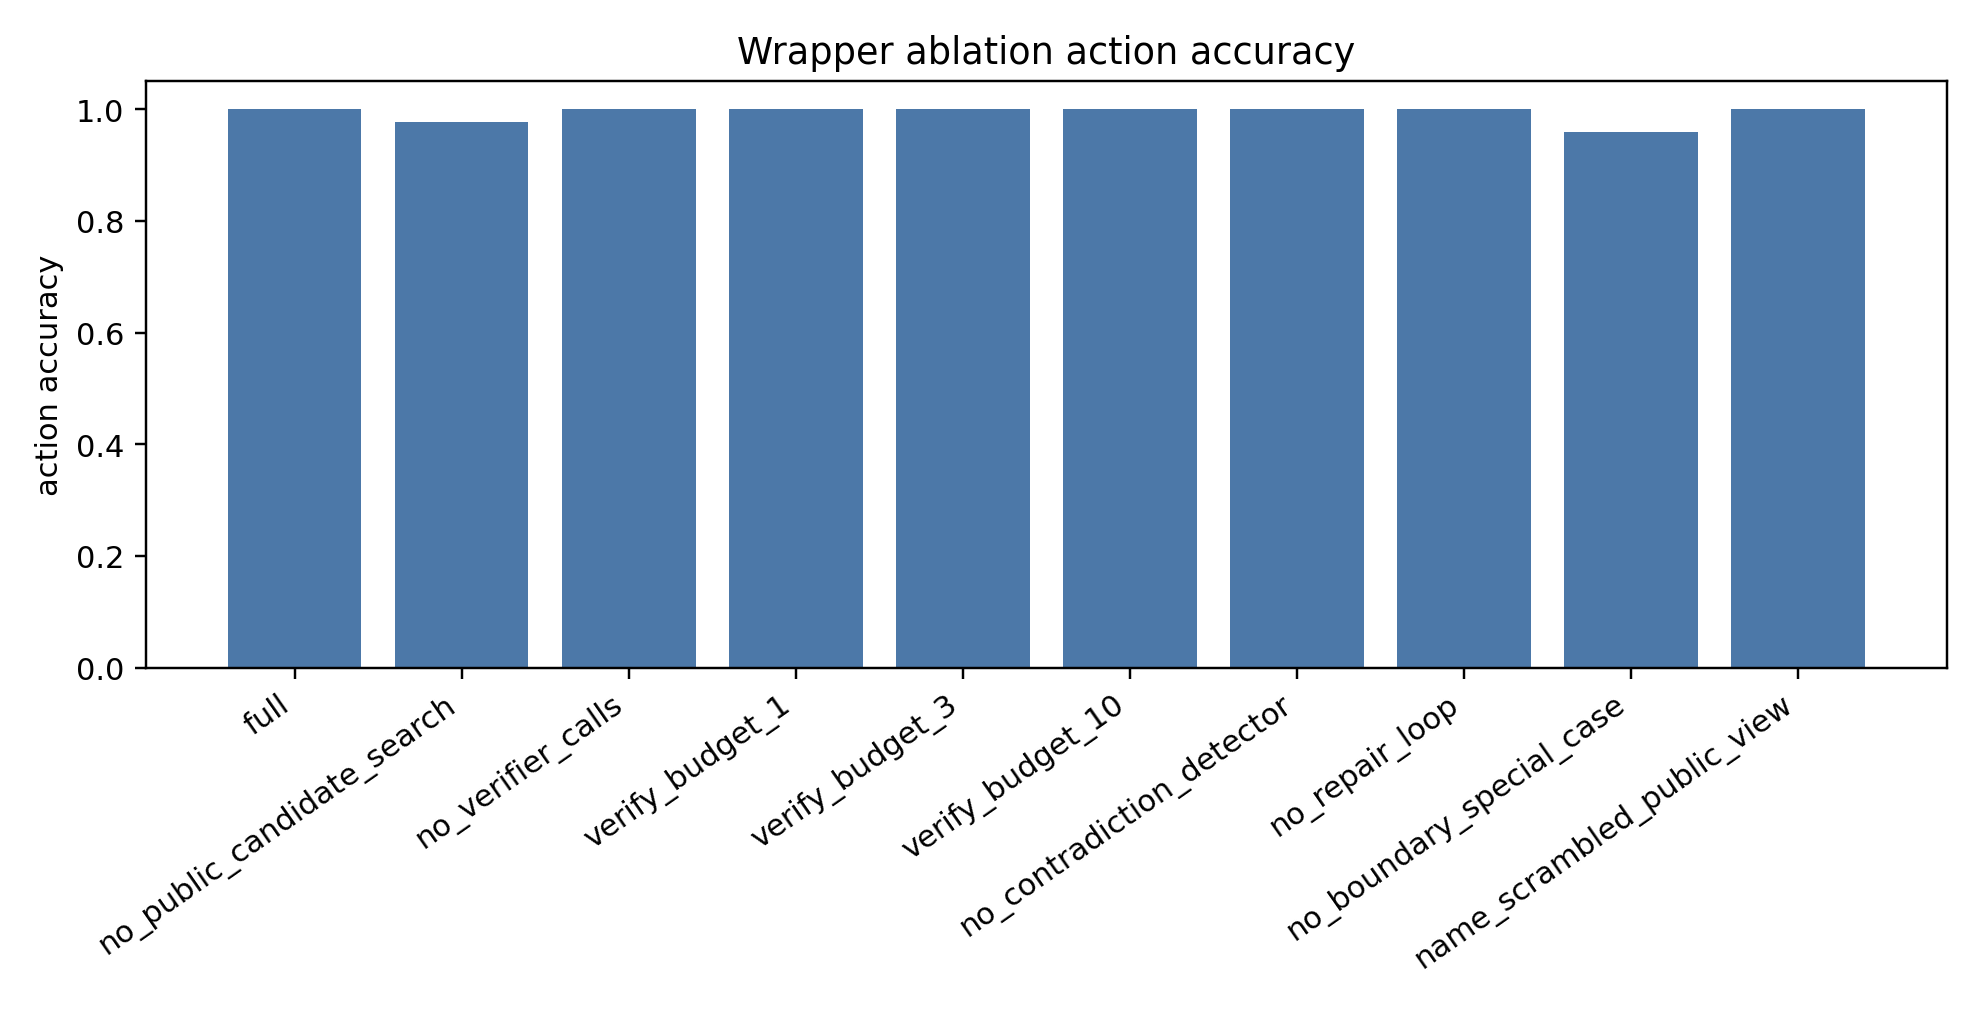
\includegraphics[width=0.85\linewidth]{figures/wrapper_ablation_action_accuracy.png}
\caption{Wrapper ablation action accuracy. The wrapper should be reported
separately from closed-book systems.}
\label{fig:wrapper}
\end{figure}

\section{Metric Sensitivity}

Metric choice changes the apparent winner. Molecule acceptance favors retrieval
and mutation systems that often accept incorrectly. Reject recall favors systems
that reject broadly. Abstain recall favors systems that abstain broadly. The
primary paper should therefore lead with action accuracy and class-specific
diagnostics rather than a single aggregate acceptance score.

\begin{figure}[htbp]
\centering
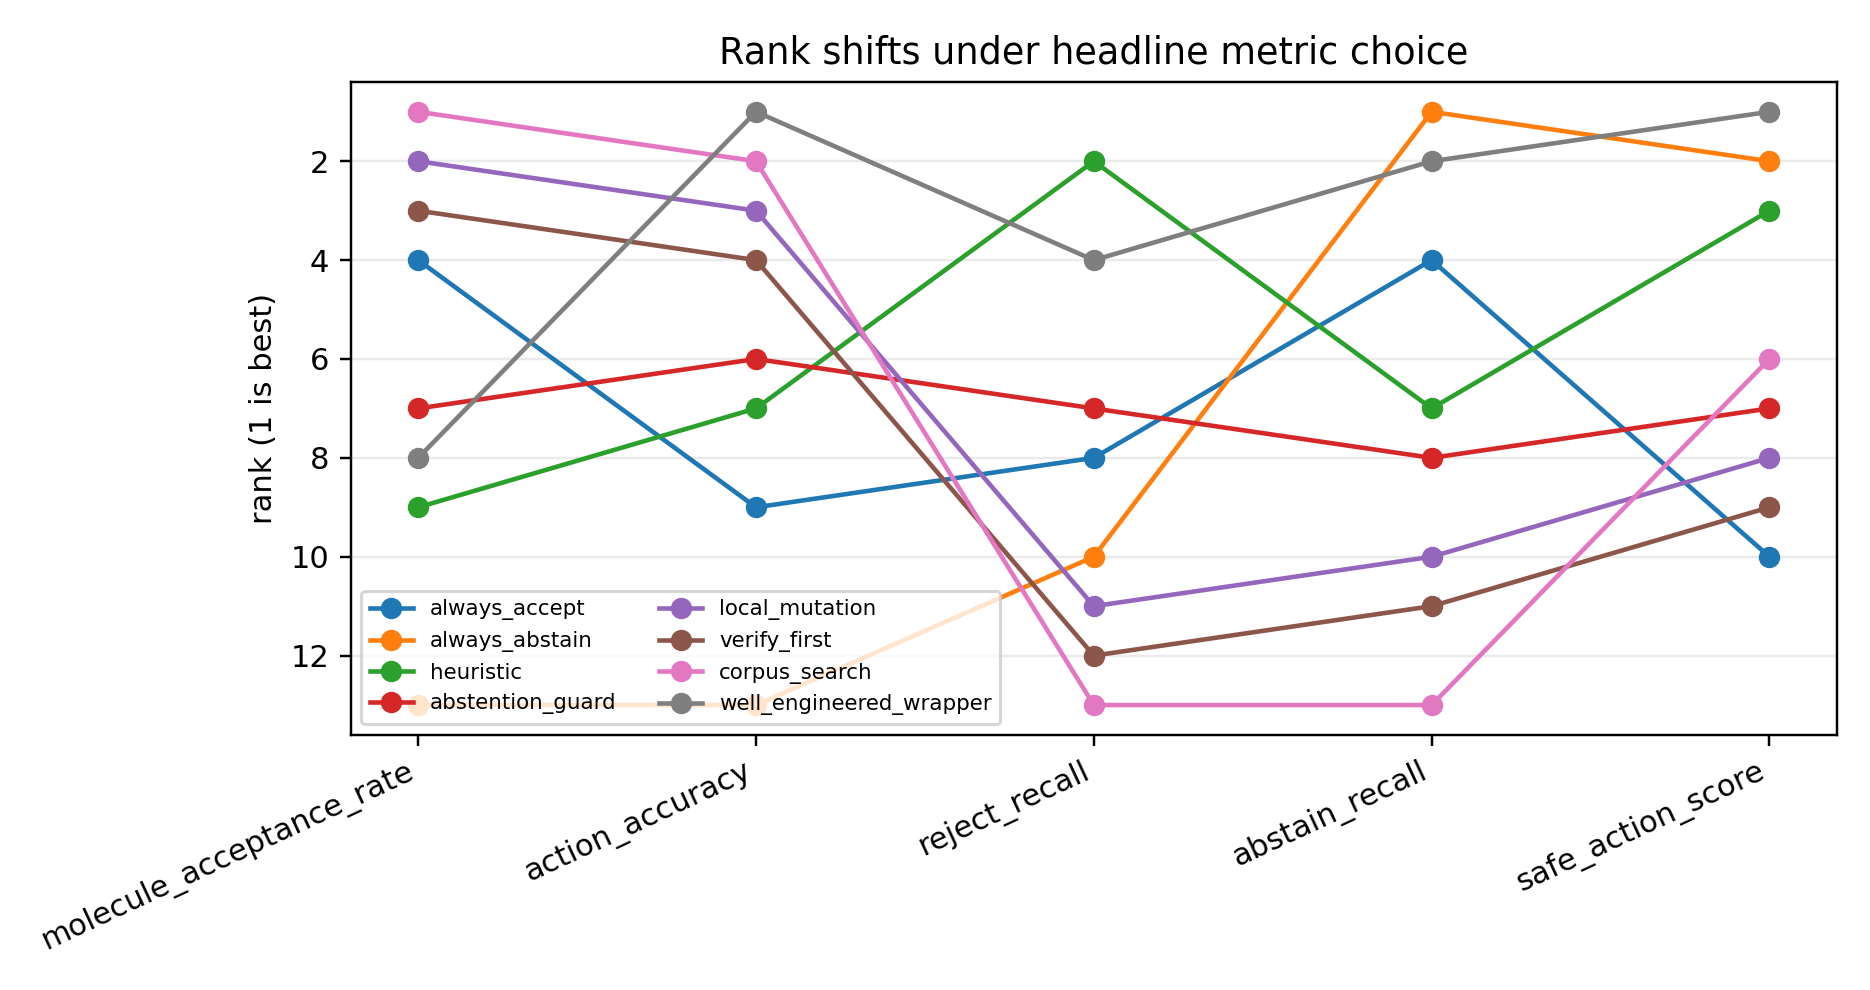
\includegraphics[width=0.95\linewidth]{figures/metric_rank_shift.png}
\caption{Metric ranking sensitivity. Different objectives produce different
apparent winners, motivating action-aware reporting.}
\label{fig:metric-shift}
\end{figure}

\section{External Baselines and Interface Contracts}

External LLM baselines should be reported as an interface evaluation, not simply
as a model leaderboard. A prompt-only JSON adapter, a provider JSON mode, a
strict schema-constrained response, and a strict tool-call interface are
different experimental conditions. Malformed JSON, fenced JSON, missing fields,
empty content, and invalid tool arguments are therefore interface failures unless
the call was made through the provider's strongest available structured-output
mechanism and still failed.

The next external run should use a tiered interface design. OpenAI baselines
should use strict JSON Schema structured outputs for final actions and function
calling for verifier interactions. Anthropic baselines should use strict tool use
with an input schema rather than free-text JSON. DeepSeek baselines should use
strict function calling when the selected model supports it, and otherwise be
reported separately as JSON-mode or prompt-JSON baselines. Each external row
should record provider, model id, model access date, interface tier, schema hash,
prompt hash, temperature, token budget, live/cache/replay status, and explicit
interface failure rates.

\begin{table}[htbp]
\centering
\caption{External-baseline interface tiers. Rows from different tiers should not
be merged into a single model leaderboard.}
\label{tab:interface-tiers}
\small
\begin{tabular}{lll}
\toprule
Tier & Mechanism & Paper interpretation \\
\midrule
prompt-json & natural-language JSON instruction only & weak interface baseline \\
json-mode & provider enforces syntactic JSON & syntax-constrained, not schema-constrained \\
strict-schema & provider enforces JSON Schema & primary final-action interface \\
strict-tool-call & provider enforces tool-call schema & primary verifier/tool interface \\
\bottomrule
\end{tabular}
\end{table}

The imported 80-task external snapshot should be read through this lens. It is
useful because it shows what went wrong in early external baselines, but it is
not a final model comparison. The deterministic subset rows reproduce the main
offline conclusion: \texttt{corpus\_search} reaches molecule acceptance 0.900
while reject and abstain recall are 0.000. Some external rows perform well on
the subset, notably \texttt{openai\_strong\_closed} with action accuracy 0.900
and balanced action accuracy 0.958. Other rows collapse to abstention or
underperform on ACCEPT tasks.

The legacy external rows are diagnostic for two reasons. First, the subset is
smaller than the held-out split. Second, the notes record interface-level
caveats: Anthropic Haiku often returned fenced JSON that an earlier strict parser
treated as invalid, and OpenAI fast had many empty cached responses. The safe
claim is not that a specific provider fails; it is that the external interface
itself must be benchmarked and controlled before model-capability claims are
made.

\begin{table}[htbp]
\centering
\caption{Legacy external diagnostic rows on the 80-task subset. These rows are
diagnostic interface evidence, not the primary benchmark leaderboard.}
\label{tab:external}
\small
\begin{tabular}{lrrrrr}
\toprule
System & Action acc. & Balanced acc. & Mol. accept & Reject rec. & Abstain rec. \\
\midrule
corpus\_search & 0.787 & 0.333 & 0.900 & 0.000 & 0.000 \\
wrapper & 1.000 & 1.000 & 0.787 & 1.000 & 1.000 \\
openai\_fast\_closed & 0.100 & 0.333 & 0.000 & 0.000 & 1.000 \\
openai\_strong\_closed & 0.900 & 0.958 & 0.688 & 1.000 & 1.000 \\
anthropic\_strong\_closed & 0.775 & 0.905 & 0.562 & 1.000 & 1.000 \\
deepseek\_fast\_verify\_l3 & 0.738 & 0.857 & 0.537 & 0.889 & 1.000 \\
deepseek\_strong\_closed & 0.175 & 0.397 & 0.062 & 0.111 & 1.000 \\
\bottomrule
\end{tabular}
\end{table}

\begin{figure}[htbp]
\centering
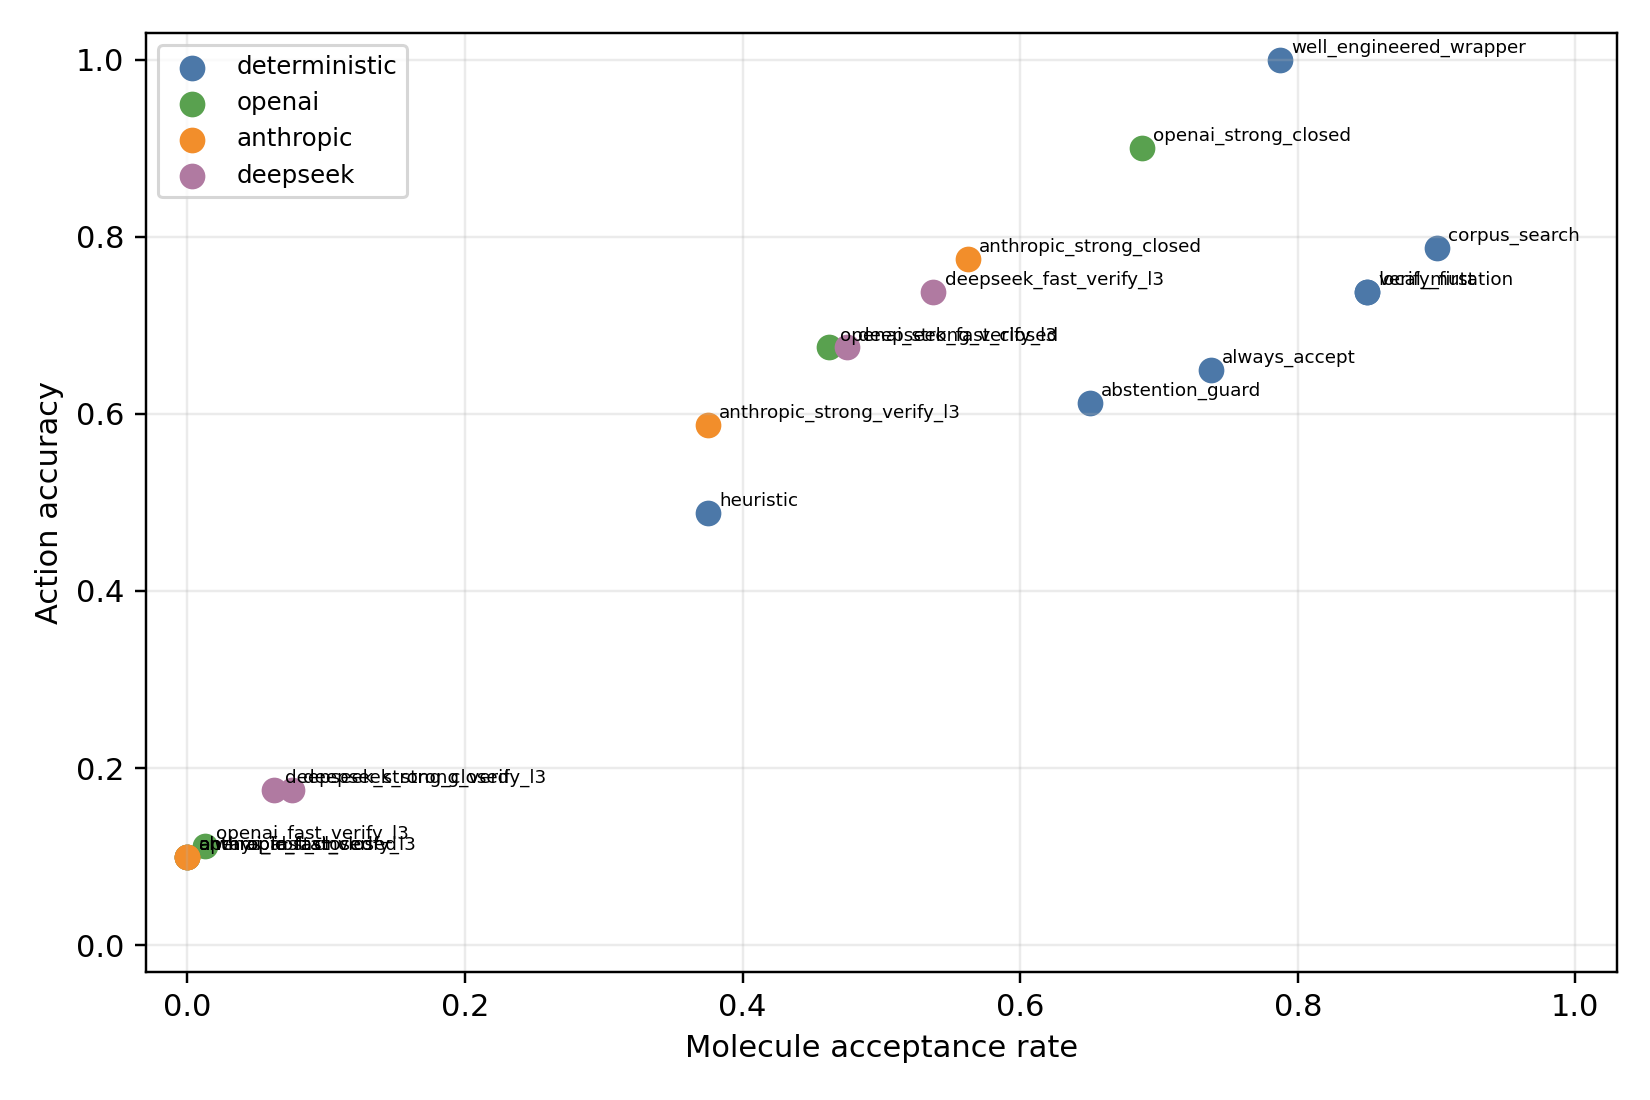
\includegraphics[width=0.85\linewidth]{figures/md_molecule_acceptance_vs_action_accuracy.png}
\caption{External-baseline subset diagnostic: molecule acceptance versus action
accuracy.}
\label{fig:md-scatter}
\end{figure}

\section{Audits and Reproducibility}

The review package preserves the generated paper_v2 validation records. The
available checks report strict validation pass, prompt-leakage audit pass,
oracle-scrambling negative controls pass, Croissant validation pass, and a
paper-v2 consistency check with zero errors and zero warnings. Because this is
not being prepared for NeurIPS submission, hosted-URL preflight is not treated as
a gating requirement. Clean-clone reproduction should still be rerun before any
public release, but it is not necessary for this internal review draft.

\section{Discussion}

SpecGuard-Chem should be revived as a paper about benchmark validity, not as a
claim that the task is intrinsically difficult for all engineered systems. The
strong result is the combination of: (i) action-aware metrics exposing failures
hidden by molecule acceptance, (ii) explicit public/private oracle boundaries,
(iii) wrapper saturation as an access-model ceiling, and (iv) external baseline
protocols that treat structured-output conformance as part of the experimental
interface. The paper is strongest when it treats wrapper saturation and interface
failure accounting as findings to report rather than flaws to hide.

\section{Review Package Contents}

The consolidated review package is under \texttt{paper\_final/}. Full source
tables are in \texttt{paper\_final/tables/}; selected paper-facing figures are in
\texttt{paper\_final/figures/}; and source memos and validation summaries are in
\texttt{paper\_final/reports/}. The original imported result packages remain at
\texttt{paper\_v2/results/} and \texttt{md\_research/results/}. The latter is
treated as a historical external-baseline diagnostic package, not as a dedicated
medicinal-chemistry project result.

\end{document}
